%%%%%%%%%%%%%%%%%%%%%%%%%%%%%%%%%%%%%%%%%
% Beamer Presentation
% LaTeX Template
% Version 2.0 (March 8, 2022)
%
% This template originates from:
% https://www.LaTeXTemplates.com
%
% Author:
% Vel (vel@latextemplates.com)
%
% License:
% CC BY-NC-SA 4.0 (https://creativecommons.org/licenses/by-nc-sa/4.0/)
%
%%%%%%%%%%%%%%%%%%%%%%%%%%%%%%%%%%%%%%%%%

%----------------------------------------------------------------------------------------
%	PACKAGES AND OTHER DOCUMENT CONFIGURATIONS
%----------------------------------------------------------------------------------------

\documentclass[
	11pt, % Set the default font size, options include: 8pt, 9pt, 10pt, 11pt, 12pt, 14pt, 17pt, 20pt
	%t, % Uncomment to vertically align all slide content to the top of the slide, rather than the default centered
	%aspectratio=169, % Uncomment to set the aspect ratio to a 16:9 ratio which matches the aspect ratio of 1080p and 4K screens and projectors
]{beamer}

\graphicspath{{Images/}{./}} % Specifies where to look for included images (trailing slash required)

\usepackage{booktabs} % Allows the use of \toprule, \midrule and \bottomrule for better rules in tables
\usepackage{cite}
\usepackage{amsmath,amssymb,amsfonts}
%\usepackage{graphicx}
\usepackage{textcomp}
\usepackage{xcolor}
\usepackage{tikz}
\usepackage{pgfplots}
\usepackage{pgfplotstable}
\usepackage{rtsched}
\usepackage{subcaption}
\usepackage{threeparttable}
\usepackage{csvsimple}
\usepackage{booktabs} % For \toprule, \midrule and \bottomrule
\usepackage{siunitx} % Formats the units and values
%\usepackage[hidelinks]{hyperref}
\usetikzlibrary{patterns,calc,arrows}
\usepackage[utf8]{inputenc}
\usepackage[T1]{fontenc}
\usepackage{pgf}
\usepackage{amsmath}
\usepackage{bm}
\usepackage{url}
%\usepackage{algorithm}
%\usepackage{algpseudocode}
\def\UrlBreaks{\do\/\do-}
\usepackage{breakurl}
%\usepackage[breaklinks,hidelinks]{hyperref}
%----------------------------------------------------------------------------------------
%	SELECT LAYOUT THEME
%----------------------------------------------------------------------------------------

% Beamer comes with a number of default layout themes which change the colors and layouts of slides. Below is a list of all themes available, uncomment each in turn to see what they look like.

%\usetheme{default}
%\usetheme{AnnArbor}
%\usetheme{Antibes}
%\usetheme{Bergen}
%\usetheme{Berkeley}
%\usetheme{Berlin}
%\usetheme{Boadilla}
%\usetheme{CambridgeUS}
%\usetheme{Copenhagen}
%\usetheme{Darmstadt}
%\usetheme{Dresden}
%\usetheme{Frankfurt}
%\usetheme{Goettingen}
%\usetheme{Hannover}
%\usetheme{Ilmenau}
%\usetheme{JuanLesPins}
%\usetheme{Luebeck}
\usetheme{Madrid}
%\usetheme{Malmoe}
%\usetheme{Marburg}
%\usetheme{Montpellier}
%\usetheme{PaloAlto}
%\usetheme{Pittsburgh}
%\usetheme{Rochester}
%\usetheme{Singapore}
%\usetheme{Szeged}
%\usetheme{Warsaw}

%----------------------------------------------------------------------------------------
%	SELECT COLOR THEME
%----------------------------------------------------------------------------------------

% Beamer comes with a number of color themes that can be applied to any layout theme to change its colors. Uncomment each of these in turn to see how they change the colors of your selected layout theme.

%\usecolortheme{albatross}
%\usecolortheme{beaver}
%\usecolortheme{beetle}
%\usecolortheme{crane}
%\usecolortheme{dolphin}
%\usecolortheme{dove}
%\usecolortheme{fly}
%\usecolortheme{lily}
%\usecolortheme{monarca}
%\usecolortheme{seagull}
%\usecolortheme{seahorse}
%\usecolortheme{spruce}
%\usecolortheme{whale}
%\usecolortheme{wolverine}

%----------------------------------------------------------------------------------------
%	SELECT FONT THEME & FONTS
%----------------------------------------------------------------------------------------

% Beamer comes with several font themes to easily change the fonts used in various parts of the presentation. Review the comments beside each one to decide if you would like to use it. Note that additional options can be specified for several of these font themes, consult the beamer documentation for more information.

\usefonttheme{default} % Typeset using the default sans serif font
%\usefonttheme{serif} % Typeset using the default serif font (make sure a sans font isn't being set as the default font if you use this option!)
%\usefonttheme{structurebold} % Typeset important structure text (titles, headlines, footlines, sidebar, etc) in bold
%\usefonttheme{structureitalicserif} % Typeset important structure text (titles, headlines, footlines, sidebar, etc) in italic serif
%\usefonttheme{structuresmallcapsserif} % Typeset important structure text (titles, headlines, footlines, sidebar, etc) in small caps serif

%------------------------------------------------

%\usepackage{mathptmx} % Use the Times font for serif text
\usepackage{palatino} % Use the Palatino font for serif text

%\usepackage{helvet} % Use the Helvetica font for sans serif text
\usepackage[default]{opensans} % Use the Open Sans font for sans serif text
%\usepackage[default]{FiraSans} % Use the Fira Sans font for sans serif text
%\usepackage[default]{lato} % Use the Lato font for sans serif text

%----------------------------------------------------------------------------------------
%	SELECT INNER THEME
%----------------------------------------------------------------------------------------

% Inner themes change the styling of internal slide elements, for example: bullet points, blocks, bibliography entries, title pages, theorems, etc. Uncomment each theme in turn to see what changes it makes to your presentation.

%\useinnertheme{default}
\useinnertheme{circles}
%\useinnertheme{rectangles}
%\useinnertheme{rounded}
%\useinnertheme{inmargin}

%----------------------------------------------------------------------------------------
%	SELECT OUTER THEME
%----------------------------------------------------------------------------------------

% Outer themes change the overall layout of slides, such as: header and footer lines, sidebars and slide titles. Uncomment each theme in turn to see what changes it makes to your presentation.

%\useoutertheme{default}
%\useoutertheme{infolines}
%\useoutertheme{miniframes}
%\useoutertheme{smoothbars}
%\useoutertheme{sidebar}
%\useoutertheme{split}
%\useoutertheme{shadow}
%\useoutertheme{tree}
%\useoutertheme{smoothtree}

%\setbeamertemplate{footline} % Uncomment this line to remove the footer line in all slides
%\setbeamertemplate{footline}[page number] % Uncomment this line to replace the footer line in all slides with a simple slide count

%\setbeamertemplate{navigation symbols}{} % Uncomment this line to remove the navigation symbols from the bottom of all slides

%----------------------------------------------------------------------------------------
%	PRESENTATION INFORMATION
%----------------------------------------------------------------------------------------
\usepackage[font=scriptsize]{caption}
\title[]{Energy aware memory allocation in real-time systems} % The short title in the optional parameter appears at the bottom of every slide, the full title in the main parameter is only on the title page

\subtitle{} % Presentation subtitle, remove this command if a subtitle isn't required

\author[]{Loïc Thomas} % Presenter name(s), the optional parameter can contain a shortened version to appear on the bottom of every slide, while the main parameter will appear on the title slide

\institute[]{LAAS CNRS \\ \smallskip  \textit{l\_thomas@insa-toulouse.fr}} % Your institution, the optional parameter can be used for the institution shorthand and will appear on the bottom of every slide after author names, while the required parameter is used on the title slide and can include your email address or additional information on separate lines

\date[\today]{\today} % Presentation date or conference/meeting name, the optional parameter can contain a shortened version to appear on the bottom of every slide, while the required parameter value is output to the title slide

%----------------------------------------------------------------------------------------
\AtBeginSection[]
{
    \begin{frame}
        \frametitle{Table of Contents}
        \tableofcontents[currentsection]
    \end{frame}
}


\begin{document}

%----------------------------------------------------------------------------------------
%	TITLE SLIDE
%----------------------------------------------------------------------------------------

\begin{frame}
	\titlepage % Output the title slide, automatically created using the text entered in the PRESENTATION INFORMATION block above
\end{frame}

%----------------------------------------------------------------------------------------
%	TABLE OF CONTENTS SLIDE
%----------------------------------------------------------------------------------------

% The table of contents outputs the sections and subsections that appear in your presentation, specified with the standard \section and \subsection commands. You may either display all sections and subsections on one slide with \tableofcontents, or display each section at a time on subsequent slides with \tableofcontents[pausesections]. The latter is useful if you want to step through each section and mention what you will discuss.

%----------------------------------------------------------------------------------------
%	PRESENTATION BODY SLIDES
%----------------------------------------------------------------------------------------

\begin{frame}{Goal of the study}
	Find a new solution for energy-aware memory allocation in real-time systems on low power microcontroller.
	\begin{enumerate}
		\item Get energy consumption data on multiple benchmark with different memory configurations (CCM-SRAM, FLASH, SRAM) on cortex M4 microcontrolers.
		\item Measure the impact of each memory allocation.
		\item Create a model to optimize the energy consumption.
		\item Find scheduling algorithms which can work for this case.
	\end{enumerate}
\end{frame}

\begin{frame}{Outline of talk}
	\tableofcontents
\end{frame}

\section{Context and introduction}

\begin{frame}{Context}
	\begin{block}{Previous work}

		\begin{thebibliography}{10}
			{\tiny
			\bibitem{} Zhishen Zhang, Yuwen Shen, Binqi Sun, Tomasz Kloda, and Marco Caccamo
			\newblock Memory allocation for low-power real-time embedded microcontroler.{\em{IEEE ETFA 2022}}
			}
		\end{thebibliography}
		\begin{itemize}
			\item Tasks' memory allocation can reduce runtime in real-time context.
		\end{itemize}
	\end{block}
	\begin{figure}
		\centering
		\includegraphics[scale=0.5]{images/boost.png}
		\caption{Results of the previous work (Runtime decrease when code run from CCM-SRAM)}
	\end{figure}
\end{frame}





\begin{frame}
    \frametitle{CCM SRAM}
	\begin{center}
		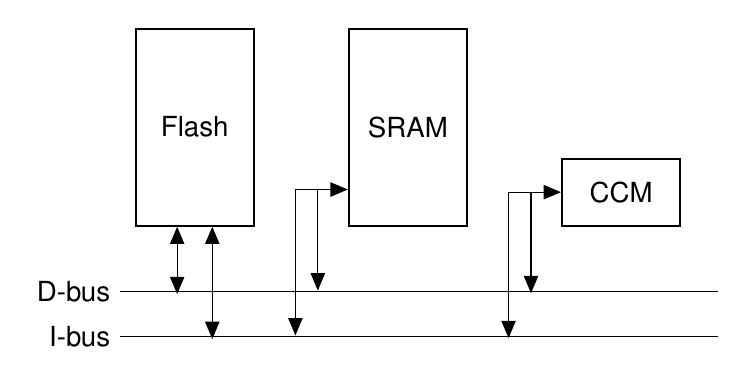
\begin{tikzpicture}[font=\sffamily,>=triangle 45,scale=0.95]
    \def\N{1}  % Number of Flip-Flops minus one
    % Place FFs
    %\foreach \m in {0,...,\N}
       %\node [shape=dff] (DFF0) at ($ 3*(0,0) $) {Flash};
     % \node [shape=dff, yscale=1.5,anchor=south] (DFF1) at ($ 3*(0.95,0) $) {SRAM};
      %\node [shape=dff, anchor=south] (DFF2) at ($ 3*(1.9,0) $) {CCM};
  
    \node (DFF0) at ($ 3*(0,0) $) [draw,thick,minimum width=1.5cm,minimum height=2.5cm, anchor=south] {Flash}; 
  
    \node (DFF1) at ($ 3*(0.95,0) $) [draw,thick,minimum width=1.5cm,minimum height=2.5cm, anchor=south] {SRAM};
  
    \node (DFF2) at  ($ 3*(1.9,0) $) [draw,thick,minimum width=1.5cm,minimum height=0.85cm, anchor=south] {CCM};
  
    % Connect FFs (Q1 with D1, etc.)
    \def\p{0}  % Used to save the previous number
    %\foreach \m in {1,...,\N} { % Note that it starts with 1, not 0
    %  \draw [->] (DFF\p.Q) -- (DFF\m.D);
    %  \global\let\p\m
    %}
  
    % Connect and label data in- and output port
    %\draw [<-] (DFF0.D) -- +(-1,0) node [anchor=east] {input} ;
    %\draw [->] (DFF\N.Q) -- +(1,0) node [anchor=west] {output};
  
    % 'Reset' port label
    %\path (DFF0) +(-2cm,+2cm) coordinate (temp)
    %  node [anchor=east] {reset};
    % Connect resets
    %\foreach \m in {0,...,\N}
    %  \draw [->] (temp) -| (DFF\m.R);
  
    % 'Set' port label
    \path (DFF0) +(-1cm,-2.2cm) coordinate (temp)
      node [anchor=east] {D-bus};
    % Connect sets
  %  \foreach \m in {0,...,2}
  %    \draw [->] (temp) -| (DFF\m.S);
       %\draw [->] (temp) -| (DFF0.S);
       \draw [<->] (DFF0.260) +(-0.0cm,-0.9cm) -- (DFF0.260);
  %     \draw [<->] ($ (DFF1.CE) + (-8mm,-2.2cm) $) -- ($ (DFF1.CE) + (-8mm,0) $) --  (DFF1.CE);
   %    \draw [<-] ($ (DFF1.CE) + (-5mm,-1.40cm) $) -- ($ (DFF1.CE) + (-5mm,-0cm) $) ;
  
          \draw [<->]  (DFF1.226) --   ($ (DFF1.226) + (-0.7cm,0cm) $) -- ($ (DFF1.226) + (-0.7cm,-1.95cm) $) ;
  
          \draw [->]  ($ (DFF1.226) + (-0.4cm,0cm) $) -- ($ (DFF1.226) + (-0.4cm,-1.35cm) $) ;
  
  
         \draw [<->]  (DFF2.180) --   ($ (DFF2.180) + (-0.7cm,0cm) $) -- ($ (DFF2.180) + (-0.7cm,-1.95cm) $) ;
  
         \draw [->]  ($ (DFF2.180) + (-0.4cm,0cm) $) -- ($ (DFF2.180) + (-0.4cm,-1.35cm) $) ;
       
     %  \draw [<->] ($ (DFF2.270) + (-8mm,-2.2cm) $) -- ($ (DFF2.CE) + (-8mm,0) $) --  (DFF2.270);
    %   \draw [<-] ($ (DFF2.CE) + (-5mm,-1.40cm) $) -- ($ (DFF2.CE) + (-5mm,-0cm) $) ;
       
       %\draw [->] (temp) -| (DFF1.C);
  %     \draw [->] (temp) -| (DFF2.C);
       
       \draw (temp) -- +(8cm,0cm);
  
    % Clock port label
    \path (DFF0) +(-1cm,-2.8cm) coordinate (temp)
      node [anchor=east] {I-bus};
    %\foreach \m in {0,...,\N}
      %\draw [->] (temp) -| ($ (DFF\m.CLK) + (-5mm,0) $) --(DFF\m.CLK);
  
    % Clock port label
    %\path (DFF0) +(-2cm,-3cm) coordinate (temp)
    %  node [anchor=east] {D-bus};
  %  \foreach \m in {0,...,2}
  %    \draw [->] (temp) -| ($ (DFF\m.Q) + (0mm,0) $) --(DFF\m.Q);
      %\draw [->] (temp) -| (DFF0.Q);
      \draw [<->] (DFF0.280) +(0.0cm,-1.50cm) -- (DFF0.280);
      
  %	\draw [->] (temp) -| (DFF2.C);
      
      \draw (temp) -- +(8cm,0cm);
  \end{tikzpicture}
	\end{center}
    The core coupled memory is a special area of memory. 
    It is connected to both instruction and data buses.
    It allows a no wait state access to memory. 
\end{frame}

\begin{frame}{Wait states}
	\begin{itemize}
	\item FLASH memory can be clocked up to 24MHz.
	\item When the CPU is faster than memory, it has to wait the memory to be ready.
	
	$\Rightarrow$ FLASH execution is interrupted by wait states. 
	\item The CCM-SRAM can transfer instructions at CPU clock rate.
	
	$\Rightarrow$ CCM-SRAM execution time is proportionnal to frequency. 
	\end{itemize} 
\end{frame}

\section{Microcontrolers features}

\begin{frame}{NUCLEO LPM01A}
	\centering
    \begin{minipage}{0.4\textwidth}
		\includegraphics[scale = 0.5]{images/lpm01a.jpeg}
	\end{minipage}
	\begin{minipage}{0.50\textwidth}
		\centering
		\begin{itemize}
			\item Consumption averaging (from 1 nA up to 200 mA)
			\item Measure acquisition at 3.2 Msamples/s max
			\item Transfer measures with USB
			\item Results presented as 2 columns .csv file (time/intensity)
		\end{itemize}
		\end{minipage}
\end{frame}

\begin{frame}
    \frametitle{STM32F303}
		\centering
		\begin{minipage}{0.4\textwidth}
            \includegraphics[scale = 0.04]{images/stm32f.jpg}
        \end{minipage}
        \begin{minipage}{0.5\textwidth}
			\centering
            \begin{itemize}
                \item Frequency up to 72 MHz 
                \item 8 kB CCM-SRAM 
                \item 16 kB SRAM
                \item 512 kB FLASH
                \item FLASH speed up to 24 MHz
                \item No dynamic voltage frequency scaling
            \end{itemize}

		\end{minipage}
\end{frame}



\begin{frame}
    \frametitle{STM32G43KB}
	\centering
    \begin{minipage}{0.4\textwidth}
		\includegraphics[scale = 0.04]{images/stm32g.jpg}
	\end{minipage}
	\begin{minipage}{0.50\textwidth}
		\centering
		\begin{itemize}
			\item Frequency up to 170 MHz 
			\item 10 kB CCM-SRAM
			\item 22 kB SRAM 
			\item 128 kB FLASH
			\item Instruction and data cache for flash \\ (32 and 8 lines of 4 x 64 bits) 
			\item Pre-Fetch feature
			\item Dynamic voltage scaling (3 modes)
			\item Two different SRAM
		\end{itemize}
		\end{minipage}
\end{frame}


\begin{frame}{STM32F possibilities}

\begin{block}{}
	Contrary to the STM32G, the STM32F do not have Dynamic Voltage Frequency Scaling (DVFS).\\
	The options are more limited, the results that we will have are the consequences of the memory allocation.
\end{block}
\begin{block}{Memory configurations }
	\begin{itemize}
		\item Instructions in FLASH, SRAM and \emph{CCM}
		\item Input data in \emph{SRAM}
		\item Read only data in FLASH, \emph{SRAM} and CCM
	\end{itemize}
\end{block}
	
\end{frame}


\section{Current measurement} % 
%------------------------------------------------
\begin{frame}
	\frametitle{First measures for current consumption}
	\begin{figure}
		\centering
        \includegraphics[scale=0.6]{images/pointer_chase_capture_mod.png}
        \caption{Intensity consumption graph for differents pointer chase executions}
	\end{figure}
\end{frame}

\begin{frame}{Final measures for current consumption}
	\begin{figure}
		\centering
        \includegraphics[scale=0.4]{images/pointer_chase30ex.png}
        \caption{Intensity consumption graph with 30 execution per memory configuration}
	\end{figure}
\end{frame}
%------------------------------------------------


\section{STM32F performances}
\begin{frame}{Absolute energy when code is in FLASH and CCM}
	\begin{figure}
		\includegraphics[scale = 0.4]{data/stm32f_v2/abs/abs_flash_energy32f.pdf}
		\includegraphics[scale = 0.4]{data/stm32f_v2/abs/abs_ccm_energy32f.pdf}
		\caption{Energy (mJ) when instructions are in FLASH and CCM (STM32F)}
	\end{figure}
	\begin{itemize}
		\item \emph{Instructions in FLASH :} $frequency \nearrow \; \; \Rightarrow \; \; energy \nearrow$
		\item \emph{Instructions in CCM : } $frequency \nearrow \; \; \Rightarrow \; \; energy \rightarrow$ 
	\end{itemize}
	To spare energy, tasks should run at low frequency in FLASH and high frequency in CCM.
\end{frame}


\section{STM32G performances}
\begin{frame}
	\frametitle{STM32G features}
	\begin{block}{Different execution modes}
		\begin{itemize}
			\item Range 1 mode (normal) : normal execution from 8 to 150 MHz.
			\item Range 1 boost mode : frequency up to 170 MHz, less wait states but higher voltage.
			\item Range 2 low power mode : frequency between 8 and 32 MHz, better consumption between these frequencies.
		\end{itemize}
	\end{block}
	\begin{block}{FLASH instruction cache}
		Allows zero wait states when instructions are in FLASH $\rightarrow$ same results as the CCM (runtime).
	\end{block}
\end{frame}

\begin{frame}{DVFS}
	\begin{figure}
		\includegraphics[scale = 0.4]{data/stm32g_v2/abs/abs_energy_flash_32g.pdf}
		\includegraphics[scale = 0.4]{data/stm32g_v2/abs/abs_energy_ccm.pdf}
		\caption{Energy (mJ) when instructions are in FLASH and CCM (STM32G)}
	\end{figure}
	\begin{itemize}
		\item Range 2 mode can significantly lower the energy consumption, but it can be used only in low frequencies.
		\item BOOST mode consume more energy to go faster in high frequencies. If the time gain is high enough it can be a good alternative to let other task run slower. 
	\end{itemize}
\end{frame}


\begin{frame}{Cache impact}
	\begin{figure}
		\includegraphics[scale = 0.35]{data/stm32g_v2/cache_impact/duration.pdf}
		\includegraphics[scale = 0.35]{data/stm32g_v2/cache_impact/energy.pdf}
		\caption{\emph{Runtime} and \emph{Energy} loss when cache is disabled}
	\end{figure}
	\begin{itemize}
		\item Different wait states levels
		\item In high frequencies the wait states reduce the global intensity
		\item With no wait state, there are the same runtime performances 
	\end{itemize}
\end{frame}

\begin{frame}{SRAM 1 and 2}
	\begin{minipage}{0.5\textwidth}
		\begin{figure}
			\includegraphics[scale = 0.35]{data/stm32g_v2/data_ram_data_ram2/intensity.pdf}
		\end{figure}
		\vspace*{-0.5cm}
		\begin{figure}
			\includegraphics[scale = 0.35]{data/stm32g_v2/data_ram_data_ram2/duration.pdf}
			\caption{\emph{Intensity} and \emph{Runtime} gain when we move data from RAM1 to RAM2 (code FLASH)}
		\end{figure}
	\end{minipage}
	\begin{minipage}{0.4\textwidth}
		\begin{itemize}
			\item The SRAM2 allows a better power consumption. 
			\item This intesity gain is not enough to compensate the runtime loss. 
		\end{itemize}
		It will be better to put data in SRAM1.
	\end{minipage}
\end{frame}

\begin{frame}{Pre-Fetch in STM32G}
	\begin{figure}
		\includegraphics[scale=0.7]{images/prefetch32g.png}
		\caption{Sequential 16-bit instructions execution (64-bit read data width)}
	\end{figure}
	Pre-fetch on the instruction bus can be used to read the next sequential instruction line from the Flash memory while the current instruction line is being requested by the CPU. 
\end{frame}

\begin{frame}{Pre-Fetch impact when cache is disabled}
	\begin{figure}
		\includegraphics[scale = 0.4]{data/stm32g_v2/pre_fetch_impact_cache_off/duration.pdf}
		\includegraphics[scale = 0.4]{data/stm32g_v2/pre_fetch_impact_cache_off/energy.pdf}
		\caption{Runtime and energy gains when pre-fetch is enabled}
	\end{figure}
\end{frame}

\begin{frame}{Pre-Fetch impact when cache is enabled}
	\begin{figure}
		\includegraphics[scale = 0.4]{data/stm32g_v2/pre_fetch_impact_cache_on/duration.pdf}
		\includegraphics[scale = 0.4]{data/stm32g_v2/pre_fetch_impact_cache_on/energy.pdf}
		\caption{Runtime and energy loss when pre-fetch is enabled}
	\end{figure}
\end{frame}

\section{Optimization model}

\begin{frame}
	\frametitle{Observations conclusion}
	\begin{block}{Comparaison with FLASH} % Block without title
		Moving instructions in CCM SRAM reduces runtime and energy consumption.
		It is almost always better to run code from CCM.
	\end{block}
	\begin{block}{Energy over frequency} % Block without title
		\begin{itemize}
			\item Energy is constant when code runs from CCM at every frequency. There are
			only advantages to run from CCM at maximum frequency.
			\item When instructions are in FLASH we can gain energy if the
			frequency is lower
		\end{itemize}
	\end{block}
\end{frame}

\begin{frame}
	\frametitle{Offline algorithm}
	Choose the best tasks to move in CCM and which one we lower the frequency
	\begin{equation*}
		\min \;  \sum_{i=1}^n \left(\sum_{{c}\,\in\,\mathcal{C}} {\frac{E_i^{{c}}}{T_i} \cdot x^{{c}}_i}\right)
	\end{equation*}
	\begin{block}{Constraint 1}
		\begin{minipage}{0.2\textwidth}
		\small
		\centering
		\begin{flalign*}
			\quad  \sum_{{c}\,\in\,\mathcal{C}}{x^{{c}}_i} = 1 \quad \forall \tau_i \in \Gamma  &&
		\end{flalign*}	
		\end{minipage}
		\begin{minipage}{0.65\textwidth}
			\small
			\begin{itemize}
				\item $\mathcal{C}$ Represent the set of all possible configuration (memory and frequency)
				\item Only one configuration can be selected per task.
			\end{itemize}
		\end{minipage}
	\end{block}	


	\begin{block}{Constraint 2}
		\begin{minipage}{0.2\textwidth}
		\small
		\centering
		\begin{flalign*}
			&\sum_{i=1}^n\sum_{{c} \in \mathcal{C}}{U_i^{{c}} \cdot x_i^{{c}}} \leq 1 &&
		\end{flalign*}	
		\end{minipage}
		\begin{minipage}{0.65\textwidth}
			\begin{itemize}
				\item The taskset has to remain schedulable over EDF.
				\item On standard confiuration the utilization is 1 $\Rightarrow $ always a solution
			\end{itemize}
		\end{minipage}
	\end{block}
\end{frame}	



\begin{frame}{Model memory constraints}
	\begin{block}{Constraints 3, 4 and 5}
		\begin{minipage}{0.25\textwidth}
		\scriptsize
		\begin{flalign*}
			& \sum_{i=1}^n \left(\sum_{c\in\mathcal{C}}^{p{=}P}
			{\left(x_i^{c} \cdot m_i^P \right)}
				+\sum_{c\in\mathcal{C}}^{ro{=}C}
			{\left(x_i^{c} \cdot m_i^{Ro} \right)}\right) \leq M^{C} &&
		\end{flalign*}	

		\begin{flalign*}
				& \sum_{i=1}^n \left(\sum_{c\in\mathcal{C}}^{p{=}F}
				{\left(x_i^{c} \cdot m_i^P \right)}
				 +\sum_{c\in\mathcal{C}}^{ro{=}F}
				{\left(x_i^{c} \cdot m_i^{Ro} \right)}\right) \leq M^{F} &&
		\end{flalign*}

		\begin{flalign*}
				& \sum_{i=1}^n \left(\sum_{c\in\mathcal{C}}^{d{=}R}
				{\left(x_i^{c} \cdot m_i^D \right)}
				 +\sum_{c\in\mathcal{C}}^{ro{=}R}
				{\left(x_i^{c} \cdot m_i^{Ro} \right)}\right) \leq M^{R} &&
		\end{flalign*}
		\end{minipage}
		\begin{minipage}{0.45\textwidth}
			\small
			\begin{itemize}
				\item Constraint on CCM, FLASH and SRAM space
				\item The sums on c cover only the case which concern the good memory 
				
				(ex : $d=R$ means that input data is in SRAM)
			\end{itemize}
		\end{minipage}
	\end{block}		

\end{frame}


\begin{frame}{Energy results on STM32F}
	\begin{figure}
		\includegraphics{data/model/poster.pdf}
		\caption{Utilization and energy gains with the model on STM32F}
	\end{figure}
	Comparing to the default configuration we can consume 20\% less energy. 
	With a low number of tasks we can even gain utilization.
\end{frame}

\begin{frame}{Frequency results on STM32F}
	\begin{figure}
        \includegraphics[scale = 0.6]{data/model/frequency_choose.pdf}
		\includegraphics[scale = 0.6]{data/model/frequency_choose_CCM.pdf}
		\caption{Frequency choices made by the model for tasks in FLASH and CCM}
	\end{figure}
The proportion of tasks in CCM decrease over the number of tasks. \\
With less tasks, the tasks in FLASH run at low or mid frequency. \\
When the number of task begin to be high more tasks in FLASH are executed at 72MHz \\
$\Rightarrow $ when the system is crowded (U $\to$ 1) it tends to the default config.
\end{frame}


\begin{frame}[fragile]
	\frametitle{ Normal EDF example }
	\begin{figure}
		\includegraphics{schedule/edf.pdf}
	\end{figure}
	We have 3 tasks in the standard configuration. \\
	Instructions are in FLASH and the CPU runs them at 72 MHz.
\end{frame}


\begin{frame}[fragile]
	\frametitle{ Application of the previous algorithm }
	\begin{figure}
		\includegraphics{schedule/offline_algo.pdf}
	\end{figure}
	We move $\tau_1$ and $\tau_2$ in the CCM 
	\\ $\Rightarrow$ runtime is reduced and consume less energy.\newline

	We use the utilization gain of the CCM to run $\tau_3$ at 48 MHz 
	\\$\Rightarrow$ runtime is bigger, but, we consume less energy. \newline

	The utilization of the system is still 1 and we spare energy.
\end{frame}

\begin{frame}{Model results on STM32G}
	\begin{figure}
		\includegraphics{data/model/results_32g.pdf}
		\caption{Utilization and energy gains with the model on STM32G}
	\end{figure}
	The default configuration use the cache so it is hard to gain utilization.\\
	We ave a better energy gain with the STM32G, with the DVFS it may be easier to consume less.
\end{frame}

\begin{frame}{Frequency results on STM32G}
	\begin{figure}
        \includegraphics[scale = 0.6]{data/model/f_choose_32g_flash.pdf}
		\includegraphics[scale = 0.6]{data/model/f_choose_32g_ccm.pdf}
		\caption{Frequency choices made by the model for tasks in FLASH and CCM for STM32G}
	\end{figure}
RANGE2 mode is even used with the CCM. 
However the boost mode is not used at all (the runtime gain is too low compared to the waste of energy).
\end{frame}


\section{Future work}
\begin{frame}
	\frametitle{Online algorithms}
	\begin{block}{Dynamic frequency and SLACK algorithm}
		If we can still complete the task with the worst case time execution before the deadline. Then we lower the frequency. 
	\end{block}
	\begin{block}{Dynamic CCM SRAM allocation}
		\begin{itemize}
			\item Divide the CCM into slots
			\item Before the execution we copy tasks' instructions in one CCM slot
			\item the worst case execution time is equal to the CCM execution time plus memory copy
			
		\end{itemize}
		$\Rightarrow$ Changes in the scheduling algorithm: mutex, blocking, non-preemptive tasks $\ldots$

	\end{block}
\end{frame}





\begin{frame}[plain] % The optional argument 'plain' hides the headline and footline
	\begin{center}
		{\Huge The End}
		
		\bigskip\bigskip % Vertical whitespace
		
		{\LARGE Questions? Comments?}
	\end{center}
\end{frame}

%----------------------------------------------------------------------------------------

\end{document} 